%!TEX root = guided_inpainting_paper.tex
\section{Introduction}
Image inpainting is the task to fill in the missing part of an image with visually plausible contents. It is one of the most typical operations of image editing~\cite{gatys2015texture} and low-level computer visions~\cite{komodakis2006image,hays2007scene}. The goal of image inpainting is to create semantically plausible contents with rich texture details, which can either be consistent with the original contents or is coherent with the known context such that the output image appears realistic. Other than image restoring and fixing, inpainting can also be used to remove unwanted objects, or in the case of guided inpainting, it can be used to composite with the contents from another image. In the latter scenario, we often need harmonization to adjust the appearance of the guidance image to make it compatible with the known context. Meanwhile, inpainting is needed to fill in the gaps between the two images.    

Traditional image inpainting methods mostly develop texture synthesis techniques to address the problem of hole-filling~\cite{bertalmio2000image,komodakis2006image,wexler2004space,barnes2009patchmatch,bertalmio2003simultaneous,wilczkowiak2005hole}. In~\cite{barnes2009patchmatch}, Barnes et al. proposes the Patch-Match algorithm which efficiently searches for the most similar patch to reconstruct the missing regions. Wilczkowiak et al.~\cite{wilczkowiak2005hole} takes further steps and detects desirable search regions to find better match patches. However, these methods only exploit the low-level signal of the known contexts to hallucinate missing regions and fall short of understanding and predicting high-level semantics. Furthermore, it is often challenging to capture the global structure of images by simply extending texture from surrounding regions. Another line of work for inpainting aims to fill in holes with content from another guidance image, by using composition and harmonization~\cite{hays2007scene,tsai2017deep}. The guidance image is often retrieved from a large database of images before it is pasted blended with the original image. Although these methods are able to propagate high-frequency details from the guidance image, they often introduce inconsistent regions and gaps which are easily detectable with human eyes.  

\begin{figure}[t]
\centering
\setlength\tabcolsep{1pt}
\begin{tabular}{ccc}
  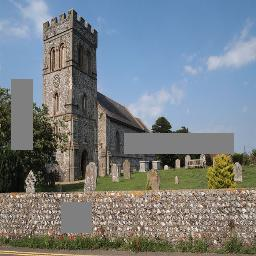
\includegraphics[width=.34\textwidth]{figures/teaser/000000120572_input_image.jpg}&
  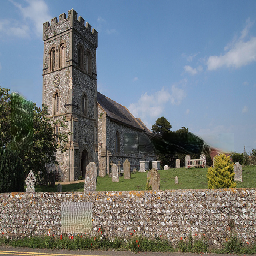
\includegraphics[width=.34\textwidth]{figures/teaser/output_mask17.png}&
  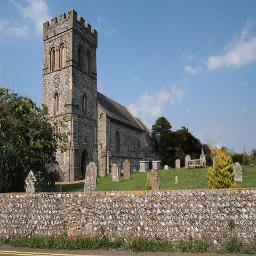
\includegraphics[width=.34\textwidth]{figures/teaser/000000120572_synthesized_image.jpg} \\
  (a) Input  & (b) GL Inpainting~\cite{iizuka2017globally} & (c) Ours  \\
  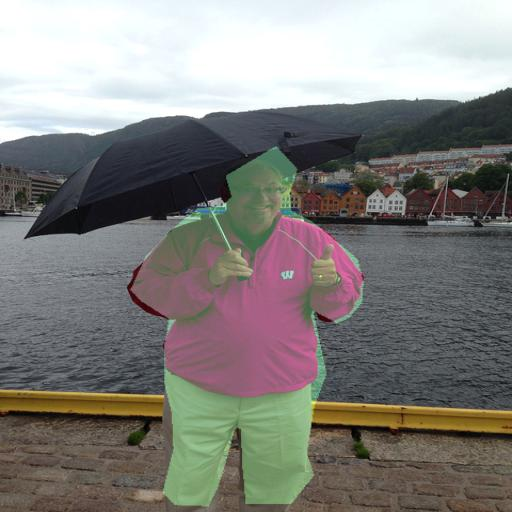
\includegraphics[width=.34\textwidth]{figures/teaser/input.jpg}&
  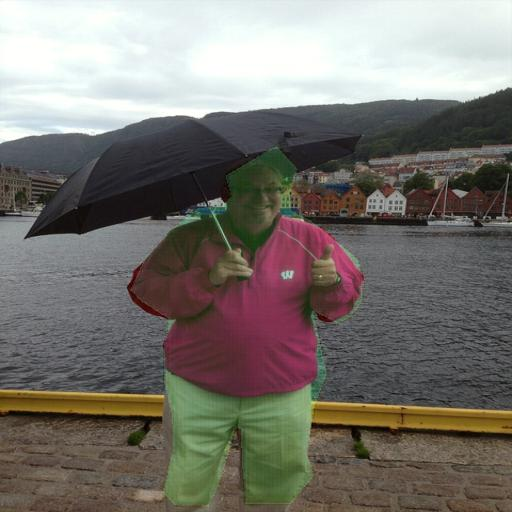
\includegraphics[width=.34\textwidth]{figures/teaser/dh.jpg}&
  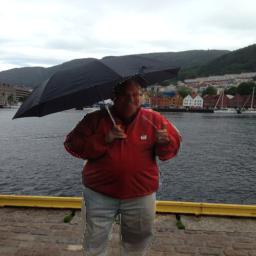
\includegraphics[width=.34\textwidth]{figures/teaser/ours.jpg} \\
  (a) Input  & (b) D~\cite{tsai2017deep} & (c) Ours  \\
\end{tabular}
\caption{An example result of inpainting (top) and harmonzation (bottom). As a general image translation framework, our approach outperforms state-of-the-art methods in both tasks (zoom in for best view). Combining inpainting and harmonization we can easily achieve image composition and guided inpainting (Sec.~\ref{exp:guided}).}
\label{fig:teaser}
\vspace{-10pt}
\end{figure}

More recently, deep neural networks have exhibited excellent performance in various computer vision tasks, including texture synthesis and image completion. In particular, adversarial training becomes the de facto strategy to train an image inpainting model~\cite{pathak2016context,yeh2016semantic,li2017generative,yang2017high,iizuka2017globally}. Pathak et al.~\cite{pathak2016context} first proposes to train an encoder-decoder model to synthesize missing holes from surrounding pixels, using both the reconstruction loss and the adversarial loss. In~\cite{yeh2016semantic}, Yeh et al. addresses inpainting by using a pre-trained model to find the most similar encoding of the corrupted image. Yang et al.~\cite{yang2017high} proposes a multi-scale neural patch synthesis approach, which optimizes the hole contents such that its feature extracted from middle layers of a pre-trained CNN matches with the features of the surrounding context. The optimization greatly improves the inpainting quality and resolution at the cost of computational efficiency. Iizuka et al.~\cite{iizuka2017globally} instead proposes a pure feed-forward model trained with global and local GANs, and generates excellent results for small holes. However, DNN based methods have several limitations. First, they are either too slow due to optimization~\cite{yang2017high} or cannot generate sufficient high-frequency details, especially for large holes~\cite{iizuka2017globally}. Second, it is difficult to handle perceptual continuity, making it necessary to resort to post-processing (e.g. Poisson blending for~\cite{iizuka2017globally}) to smooth out the coalescing regions.

In practice, we found that directly training a very deep generative network to synthesize high-frequency details is difficult. Most often we fail to stabilize the training process and the results are either overly smooth or containing significant noise and artifacts. To overcome this limitation, we discuss a new approach that produces high-quality inpainting results for various inpainting tasks, refer to as \textbf{B}lock-wise \textbf{T}rained \textbf{G}enerative \textbf{M}odel for \textbf{I}npainting (BTGMI). More specifically, we decompose the generator into a ResNet head followed by multiple refinement residual blocks. For the first phase, we train the \textbf{ResNet head} for inpainting until it converges. Then we add residual blocks one at a time. Each time we train with an additional block, we use skip connections to initialize with the trained network and gradually increase the weight of the new block. This introduces the new block gradually, forcing it to refine from the previous results and learn to generate richer details. In addition, we observe that it is essential to steadily reduce the weight of the generator adversarial loss during block-wise refinement. We refer to this training scheme as \textbf{A}dversarial \textbf{L}oss \textbf{A}nnealing (ALA).  Intuitively, AAL is helpful as the adversarial loss usually dominates in the end phase of training and the generator will falsely create noise patterns to foul the discriminator. Finally, Zhang et al.~\cite{zhang2018unreasonable} shows that the perceptual similarity, measured by internal activations of networks trained for high-level classification tasks, corresponds to human perceptual judgment far better than commonly used metrics such as the Euclidean distance. Inspired by this finding, we introduce a novel \textbf{P}atch \textbf{P}erceptual \textbf{L}oss (PPL), which penalize the perceptual difference between the inpainted patch and the original patch. Different from the perceptual losses ,used in style transfer~\cite{johnson2016perceptual,gatys2016image} and image synthesis~\cite{dosovitskiy2016generating,chen2017photographic}, we compute the feature disparity across all layers. In our experiment, we found that PPL works better than the reconstruction loss and the general perceptual loss. 

To evaluate the proposed inpainting approach, we conduct extensive experiments on different datasets. We also show that our model, although being designed for inpainting, can be used for general image translation tasks including image harmonization and composition. This enables us to jointly train inpainting with those tasks and makes it suitable for a wide range of inpainting scenarios such as object removal and guided inpainting. As shown by visual results and user-study, our network already outperforms state-of-the-art inpainting and harmonization methods without using block-wise refinement. By leveraging block-wise training, it can further add high-frequency details and eliminate the perceptual discontinuity (Fig.~\ref{fig:teaser}). Finally, we demonstrate our approach is both effective and simple to use in several real-world use cases. 

In summary, in this paper we present:
\begin{enumerate}
\item The Block-wise Trained Generative Model for Inpainting (BTGMI) as a novel, end-to-end model that generates state-of-the-art image inpainting and image composition results.  
\item Two novel training losses specifically designed for the inpainting task: the Patch Perceptual Loss (PPL) and the Multi-Scale Patch Adversarial Loss (MSPAL). We also introduce Adversarial Loss Annealing (ALA) as a new training scheme that improves the inpainting quality. 
\item Effectiveness of our approach in practical use cases, including distractor removal and guided inpainting. 
\end{enumerate}